\section{実験}
実験には10クラスの手書き数字文字画像からなるデータセットであるMNISTを使用した.
データセットは$32\times 32$ピクセルの8ビットグレースケール画像からなる.
本実験では,データセットのうち1000枚をテスト用データに割り当てた.
学習用データの画像枚数は100, 200, 300, 400, 500, 1000 と変化させた.
本研究では,パワースペクトルの使用が分類精度にどう影響するか,また錐制約部分空間法は他の分類器と比較してどのような特徴を持つのか,に焦点を当てる.
したがって,分類に使用する特徴は,畳み込み辞書学習における係数マップおよび畳み込み辞書学習における係数マップのパワースペクトルの2種類で比較する.
また,分類器については,NMFで構成された錐での錐制約部分空間法,包括凸錐による錐制約部分空間法に加えて,3層ニューラルネットワーク,Support Vector Machine (SVM)を分類器として使用した.


\begin{figure}[htb]
	\centering
	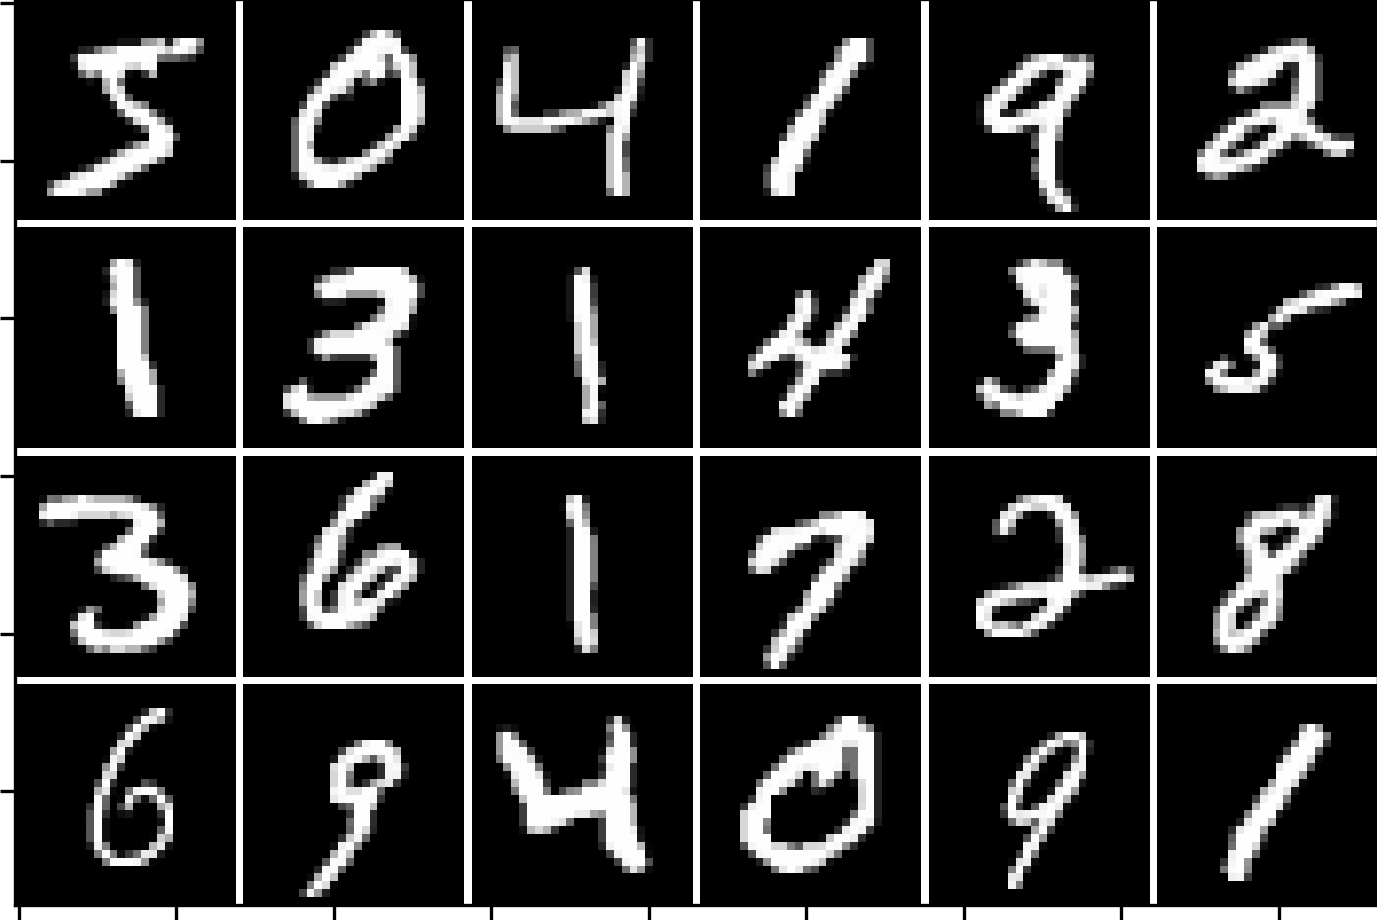
\includegraphics[width=0.7\linewidth]{image/mnist_sample.png}
	\caption{MNISTデータセットの一部}
	\label{fig:mnistsample}
\end{figure}

以下に実験の手順を示す.
先ず,学習データについて畳み込み辞書学習を行い,フィルタを設計及び,学習データの係数マップを得る.本実験では$6$枚の$5\times 5$ピクセルのフィルタを学習させた.
ここで,係数マップのパワースペクトルを特徴として使用する場合は,パワースペクトルを算出後にベクトル化する(係数マップを特徴として用いる場合はそのままベクトル化する).
これらをNMFにより256次元まで次元削減し,それらを特徴ベクトルとする.
各クラスの特徴ベクトルを用いて,錐制約部分空間法及び3層ニューラルネットワーク,SVMを学習させる.

次に,テストデータについて係数を算出する.
具体的には問題(\ref{x-update})を解くのだが,フィルタは学習データで行った畳み込み辞書学習で得られたものを使用する.
また,学習データについてと同様の操作で256次元の特徴ベクトルを得る.
最後に,学習させた各分類器で分類を行い分類精度を算出する.


なお,畳み込み辞書学習の計算にはPythonと,Python用のライブラリSPORCO\cite{sporco}を用いた.

\section{実験結果}
各学習用画像の枚数に対する実験結果を図\ref{result_first}から図\ref{result_last}に示す.
結果より,どの分類器を用いた実験においても,係数のパワースペクトルを特徴として使用すると認識精度が向上することが分かる.
これは画像中の位置ずれを,周波数の使用により吸収したためと考えられる.
また,学習枚数が比較的少ない100枚,200枚,300枚の実験では錐制約部分空間法を用いた場合が最も良い精度であり,データの数が大きくなるにつれてニューラルネットやSVMを用いた方が精度が良くなることがることから,錐制約部分空間法は学習データが少ない状況下で有効な分類器といえる.

\begin{figure}[htbp]
	\begin{minipage}{0.5\hsize}
		\begin{center}
			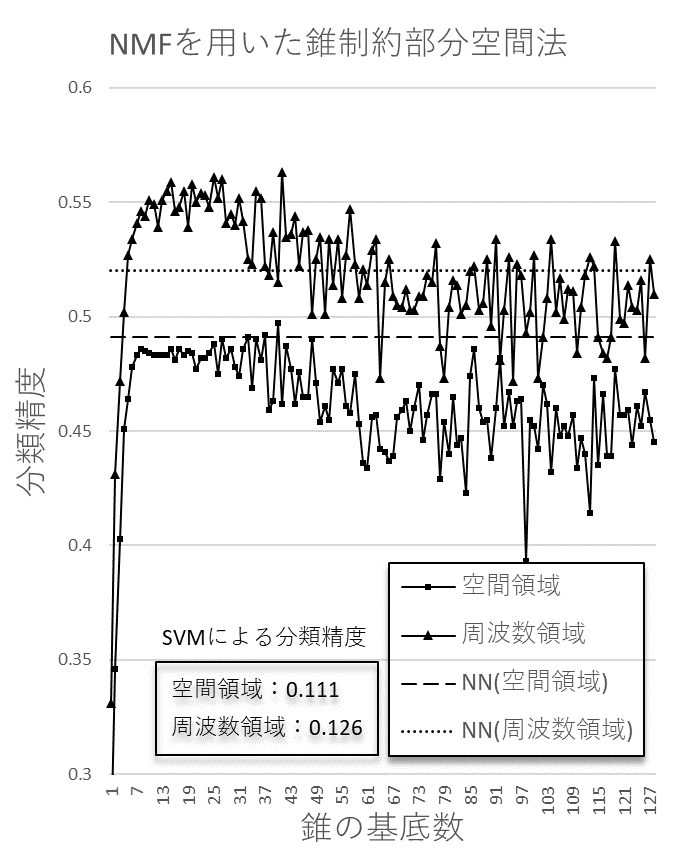
\includegraphics[width=70mm]{result/100-nmf.png}
		\end{center}
		%\caption{一つめの図}
		%\label{fig:one}
	\end{minipage}
	\begin{minipage}{0.5\hsize}
		\begin{center}
			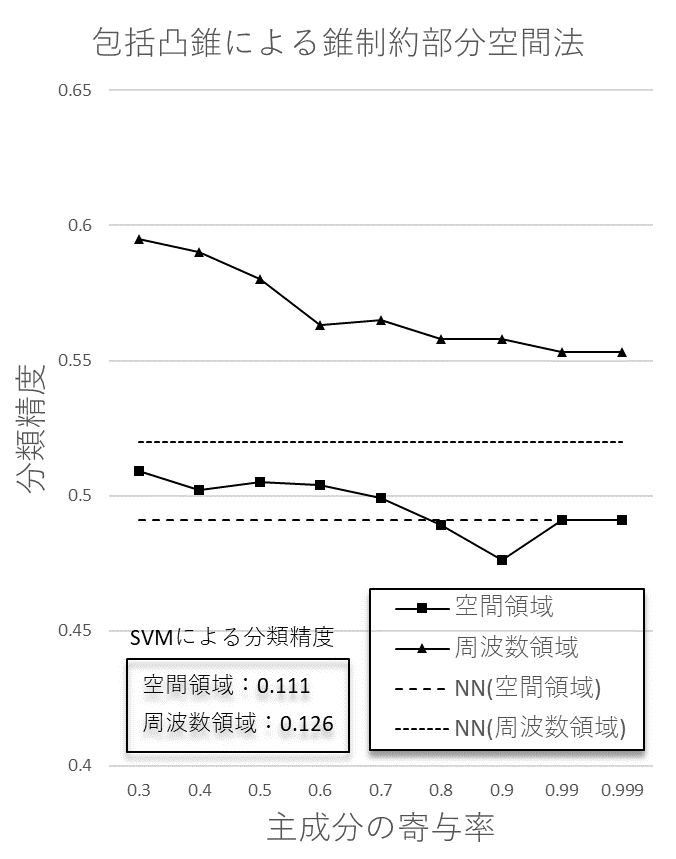
\includegraphics[width=70mm]{result/100-comp.png}
		\end{center}
		%\caption{二つめの図}
		%\label{fig:two}
	\end{minipage}
\caption{学習枚数100枚における分類精度}
\label{result_first}
\end{figure}

\begin{figure}[htbp]
	\begin{minipage}{0.5\hsize}
		\begin{center}
			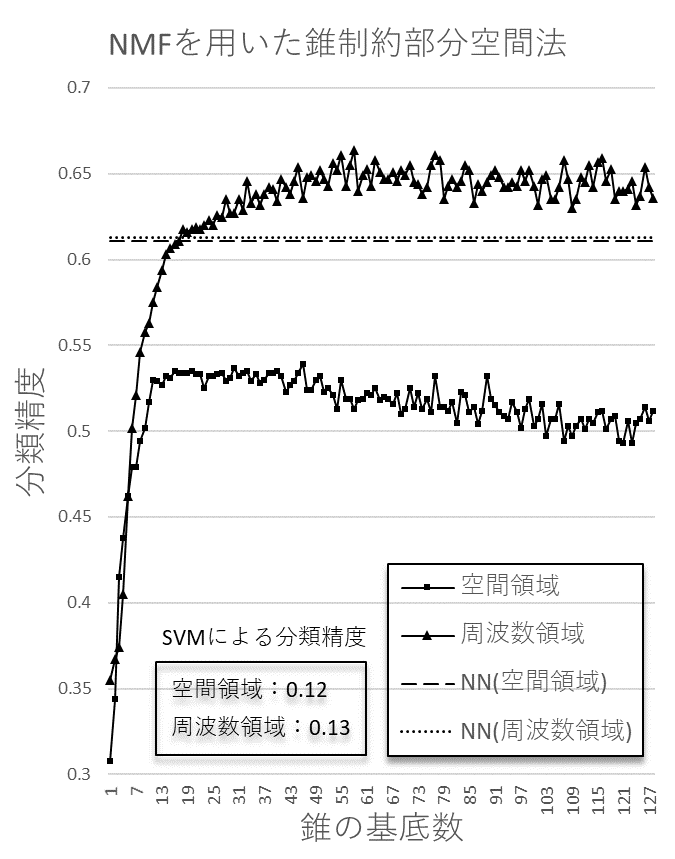
\includegraphics[width=70mm]{result/200-nmf.png}
		\end{center}
		%\caption{一つめの図}
		%\label{fig:one}
	\end{minipage}
	\begin{minipage}{0.5\hsize}
		\begin{center}
			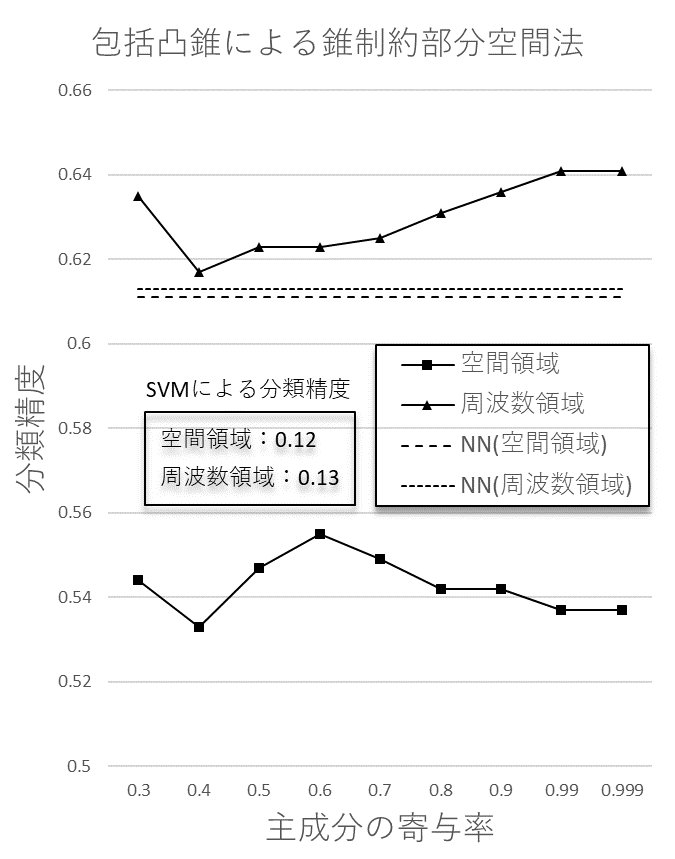
\includegraphics[width=70mm]{result/200-comp.png}
		\end{center}
		%\caption{二つめの図}
		%\label{fig:two}
	\end{minipage}
	\caption{学習枚数200枚における分類精度}
\end{figure}

\begin{figure}[htbp]
	\begin{minipage}{0.5\hsize}
		\begin{center}
			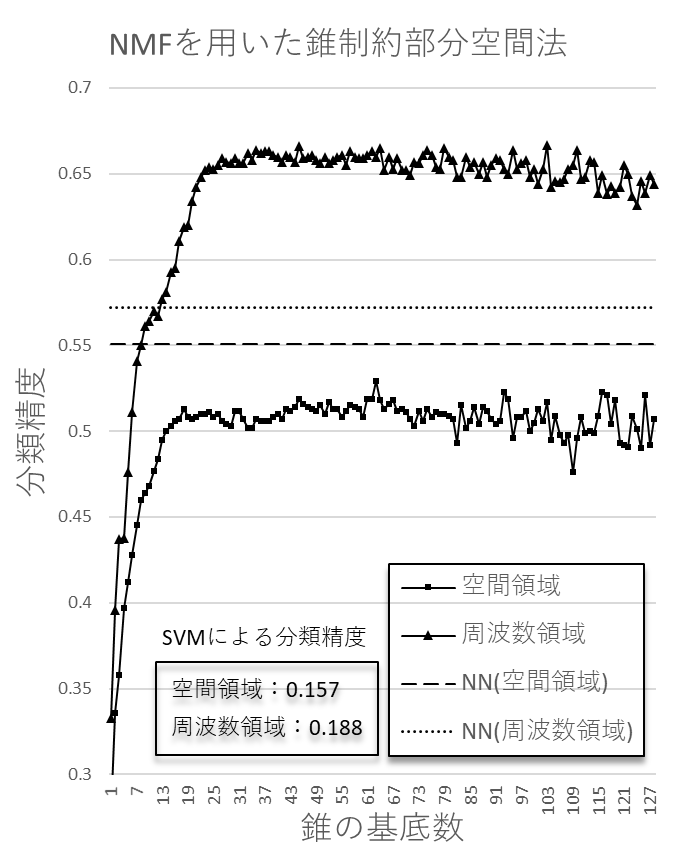
\includegraphics[width=70mm]{result/300-nmf.png}
		\end{center}
		%\caption{一つめの図}
		%\label{fig:one}
	\end{minipage}
	\begin{minipage}{0.5\hsize}
		\begin{center}
			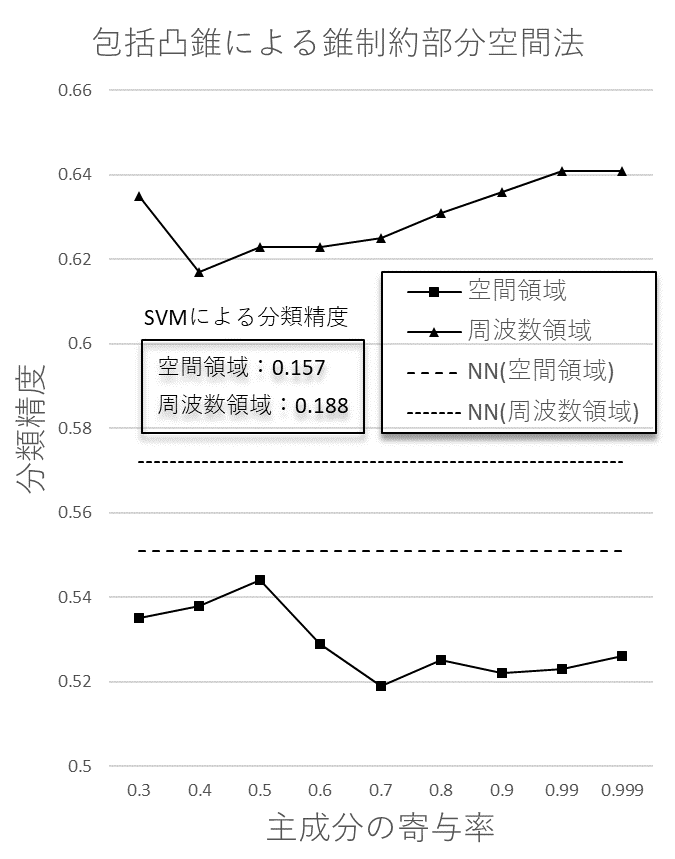
\includegraphics[width=70mm]{result/300-comp.png}
		\end{center}
		%\caption{二つめの図}
		%\label{fig:two}
	\end{minipage}
	\caption{学習枚数300枚における分類精度}
\end{figure}

\begin{figure}[htbp]
	\begin{minipage}{0.5\hsize}
		\begin{center}
			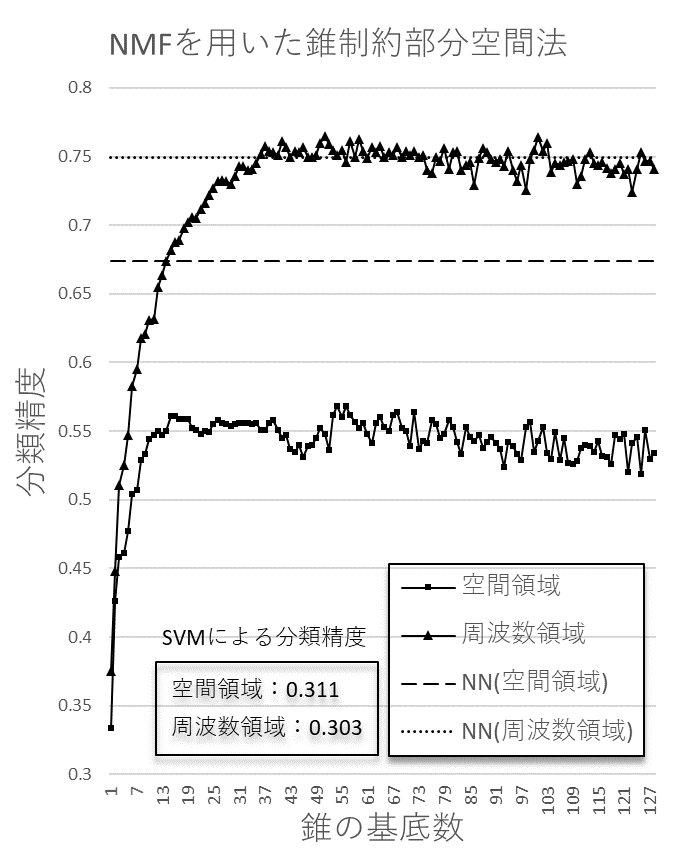
\includegraphics[width=70mm]{result/400-nmf.png}
		\end{center}
		%\caption{一つめの図}
		%\label{fig:one}
	\end{minipage}
	\begin{minipage}{0.5\hsize}
		\begin{center}
			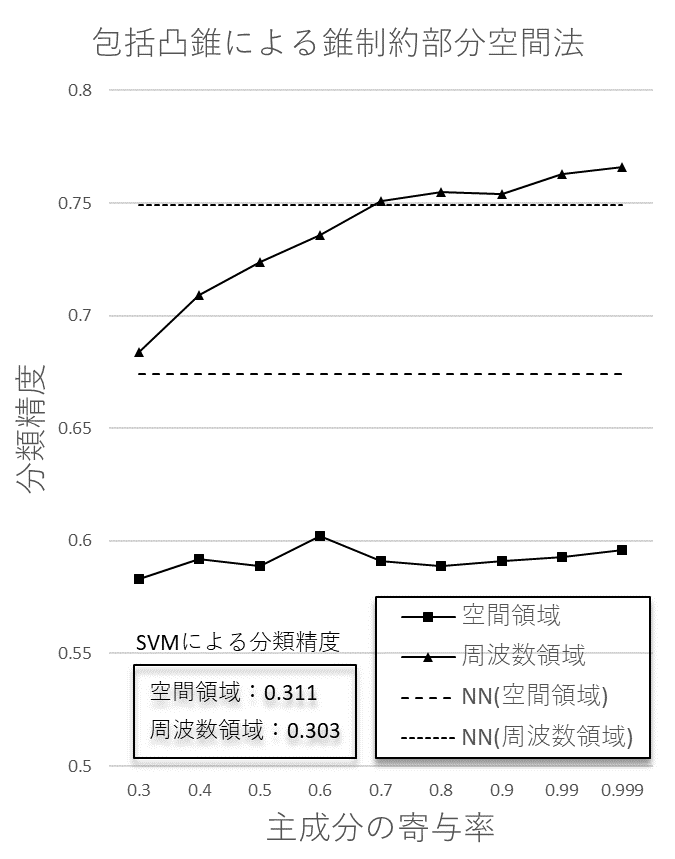
\includegraphics[width=70mm]{result/400-comp.png}
		\end{center}
		%\caption{二つめの図}
		%\label{fig:two}
	\end{minipage}
	\caption{学習枚数400枚における分類精度}
\end{figure}

\begin{figure}[htbp]
	\begin{minipage}{0.5\hsize}
		\begin{center}
			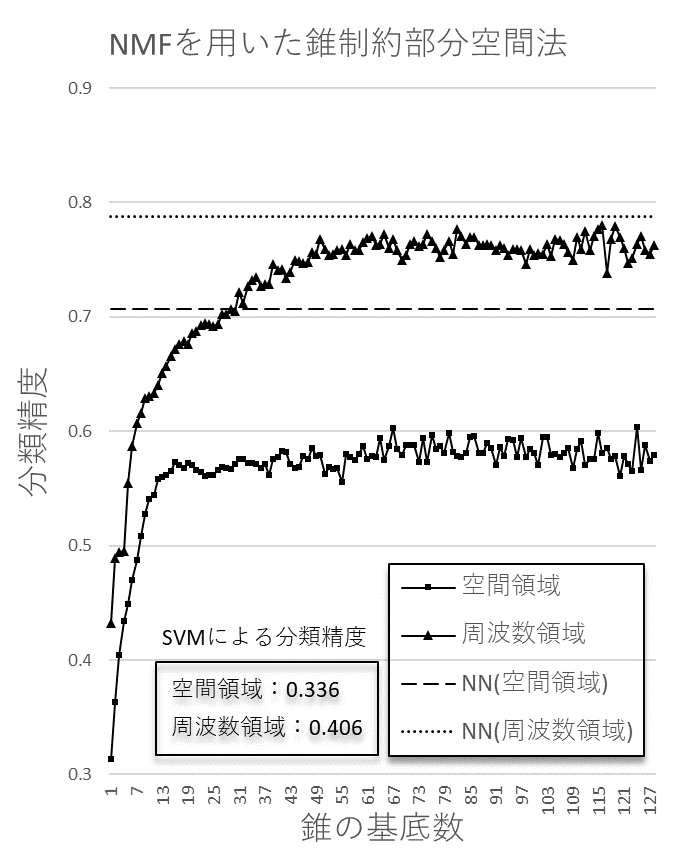
\includegraphics[width=70mm]{result/500-nmf.png}
		\end{center}
		%\caption{一つめの図}
		%\label{fig:one}
	\end{minipage}
	\begin{minipage}{0.5\hsize}
		\begin{center}
			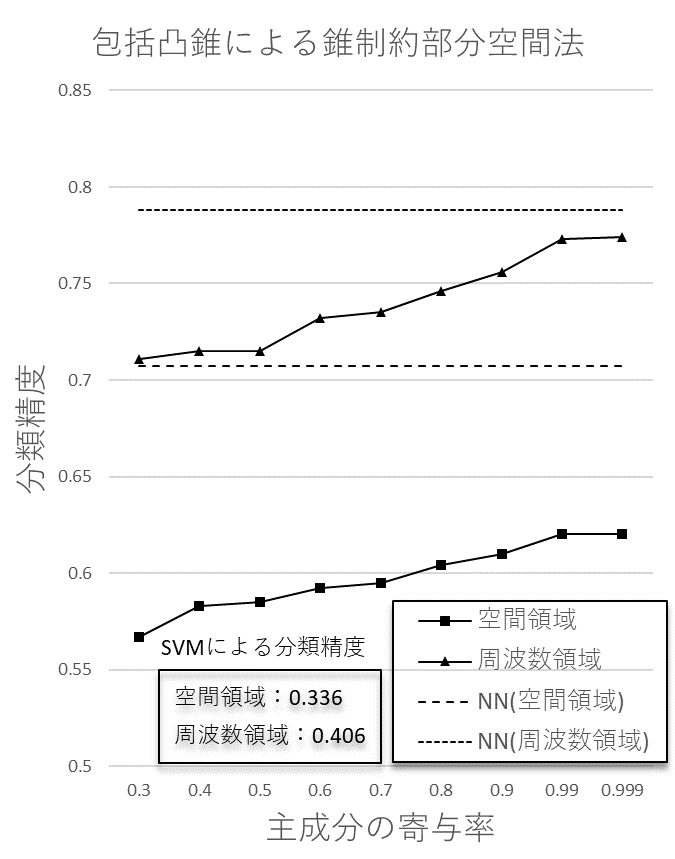
\includegraphics[width=70mm]{result/500-comp.png}
		\end{center}
		%\caption{二つめの図}
		%\label{fig:two}
	\end{minipage}
	\caption{学習枚数500枚における分類精度}
\end{figure}

\begin{figure}[htbp]
	\begin{minipage}{0.5\hsize}
		\begin{center}
			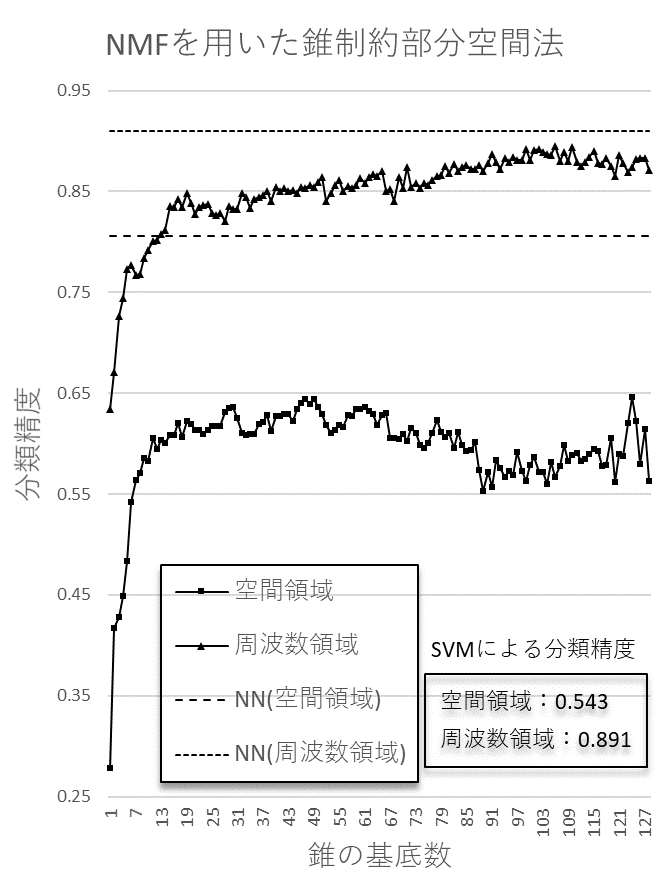
\includegraphics[width=70mm]{result/1000-nmf.png}
		\end{center}
		%\caption{一つめの図}
		%\label{fig:one}
	\end{minipage}
	\begin{minipage}{0.5\hsize}
		\begin{center}
			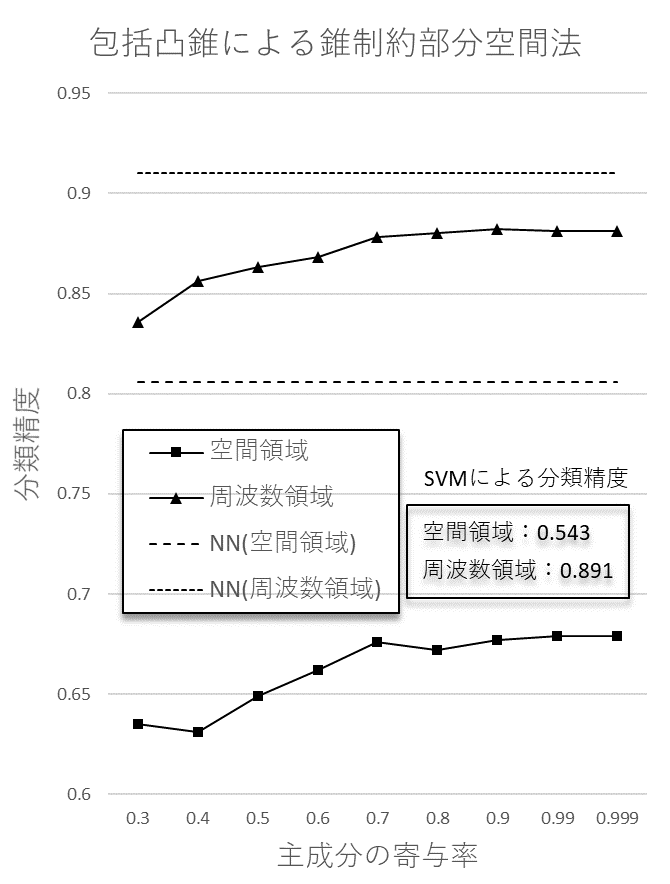
\includegraphics[width=70mm]{result/1000-comp.png}
		\end{center}
		%\caption{二つめの図}
		%\label{fig:two}
	\end{minipage}
	\caption{学習枚数1000枚における分類精度}
	\label{result_last}
\end{figure}
